\begin{frame}
   The format:
   \begin{itemize}[<+(1)->]
      \item five regular rounds
      \begin{itemize}
         \item eight questions each, which we will go through together
         \item questions within each round are linked by some common thread
      \end{itemize}
      \item picture and puzzle rounds
      \begin{itemize}
         \item for you to complete in your spare time
         \item examples to follow
      \end{itemize}
   \end{itemize}

   \onslide<8->{The etiquette:}
   \begin{itemize}[<+(1)->]
      \item if you need something clarified, just ask!
      \item at the end of each round I can repeat previous questions upon request, so don't worry if you've forgotten what a previous question was
      \item the quizmaster is \emph{always} right
   \end{itemize}
\end{frame}

\begin{frame}
   Example picture

   \begin{center}
      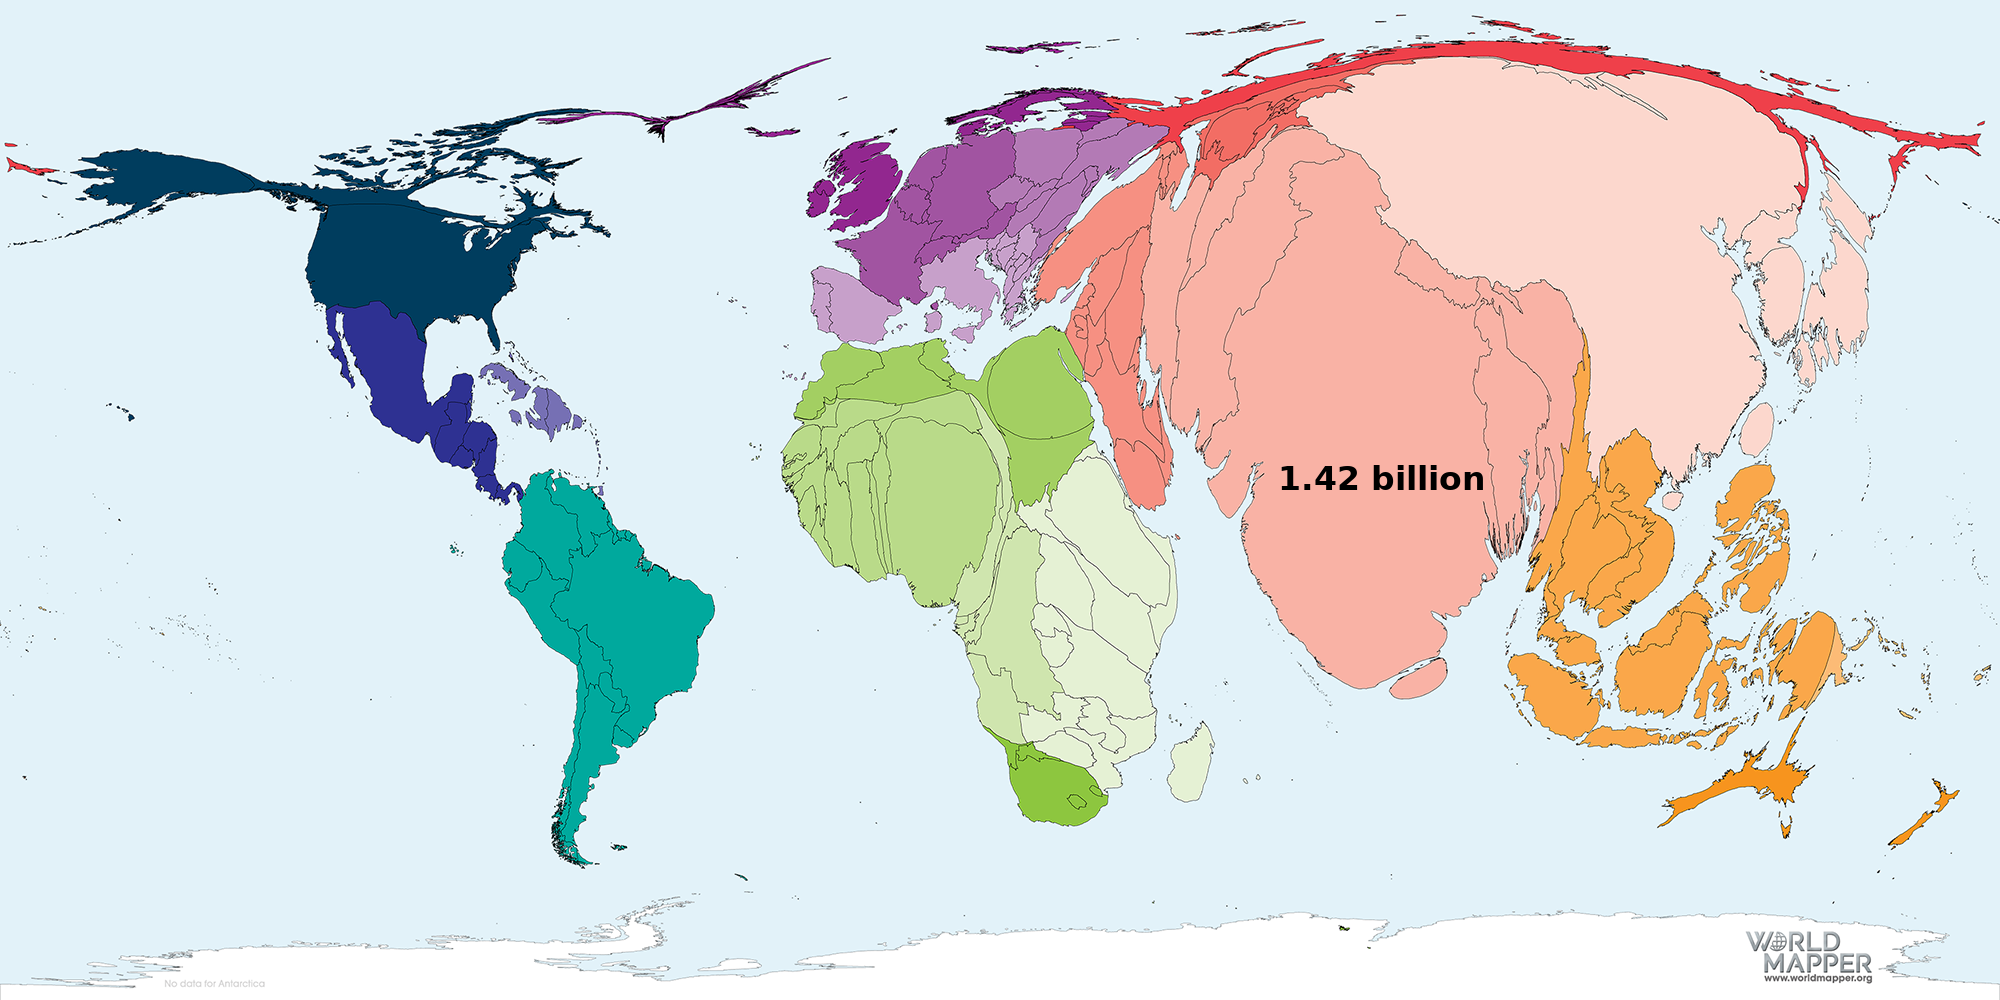
\includegraphics[width=0.6\paperwidth]{maps/population.png}

      \onslide<2->{population}
   \end{center}
\end{frame}

\begin{frame}
    \large
    Example puzzle 1. What links
          \begin{center}
                  magic, hugo, alfa, california
          \end{center}
   \onslide<2->{\textit{They all combine with a word from the NATO alphabet: Magic Mike, Victor Hugo, Alfa Romeo, and Hotel California}}
\end{frame}

\begin{frame}
   \large
   Example puzzle 2. What links
   \begin{center}
      \begin{minipage}{0.6\textwidth}
          \textit{%
              pe (skateboarding) \onslide<3->{= half-pi\textbf{pe}} \\
              thon (athletics) \onslide<4->{= half mara\textbf{thon}} \\
              son (wrestling) \onslide<5->{= half nel\textbf{son}} \\
              ley (tennis) \onslide<6->{= half-vol\textbf{ley}}}%
      \end{minipage}
   \end{center}

   \onslide<2->{Halves}%

\end{frame}
